
%%%%%%%%%%%%%%%%%%%%%%%%%%%%%%%%%%%%%%%%%%%%%%%%%%%%%%%%%%%%%%%%%%%%
\section{DAQ Design}
\label{sec:fdsp-daq-design}

\metainfo{16 Pages}


%%%%%%%%%%%%%%%%%%%%%%%%%%%%%%%%%%%
\subsection{Overview (Giles Barr)}
\label{sec:fdsp-daq-ltr}

%Here we describe the overall readout and data acquistion
%strategy. This will include the high-level data flow diagram,
%(Figure~\ref{fig:daq-readout-buffering-baseline} may be sufficient)
%which is divided in functional boxes, each of which are described in
%turn in the sections below.

The design for the \dword{daq} has been driven by finding a cost
effective solution that satisfies the requirements. Several design
choices have nevertheless been made. 
From a hardware perspecive, the DAQ design follows a standard HEP
experiment design, with customised hardware at the upstream, feeding
and funnelling (merging) and moving the data into computers. 
Once the data and triggering information are in computers, a
considerable degree of flexibility is available and the processing
proceeds with a pipelined sequence of software operations, involving
both parallel processing on multi-core computers and switched
networks. The flexibility allows the procurement of computers and
networking to be done late in the delivery cycle of the DUNE
detectors, to benefit from increased capability of commercial devices
and falling prices.

Since DUNE will operate over a number of decades, the DAQ has been
designed with upgradability in mind.  With the fall in cost of serial
links, a guiding principle is to include enough output bandwidth to
allow all the data to be passed downstream of the custom hardware.
This allows the possibility for a future very-fast farm of computing
elements to accommodate new ideas in how to collect the DUNE data.  The
high output bandwidth also gives a risk mitigation path in case the
noise levels in a part of the detector are higher than specified and
higher than tolerable by the baseline trigger decision mechanism; it
will allow additional data processing to be added (at additional cost).

The data will be collected from the TPC and photon-detector readout
systems of the single-phase and dual-phase \dwords{detmodule}. 
These partitions are viewed as essentially four types of
\dwords{submodule} within the DAQ and will follow the same overall
data collection scheme as shown in figure 1. 
The readout is arranged in a hierarchical manner to allow localized
\dword{trigdecision} to be made at the \dword{detunit} level, at the
cavern level before being combined over the full four caverns. 
The control of the detector elements will allow a fault in one part to
not halt data taking in another part, certainly at the per-cavern
level, but maybe also at more local levels. 
This will prevent a supernova burst following a failure in some part
of a cavern from being missed.

\metainfo{The folowing text will need considerable revision to make
  sure it corresponds with whatever ends up as figure 1, but the text
  here gives an idea that the overview will be a very quick visit of
  everything, and all the detail is in the later sections. 
  Note, migrated \textbf{boldface} terms to ``DUNE Words'' (bv).}

It is helpful, on first looking at the DUNE DAQ dataflow scheme, to
consider how the main data is collected first and then to look at how
the triggering and synchronization functions are included; we take
this approach in this overview. 
The main data are initially merged within one \dword{detunit} (eg, one
APA) and placed in a \dword{ringbuffer} to allow \dwords{trigdecision}
to be made. 
When a \dword{trigdecision} is performed it results in all data in a
determined time window and in a designated region of interest (ROI) as
specified by the \dword{trigcommand} to be extracted from the
\dword{ringbuffer} and sent for event building, \dword{diskbuffer} and
possible transfer to permanent storage at Fermilab. 
This covers trigger decisions for the purpose of collecting data
covering interactions of beam and atmospheric neutrino, cosmic rays,
individual supernova neutrinos and also candidates for searches such
as proton decays, or low energy events such as solar and diffuse
supernova neutrinos as well as sources of calibration. 
Additionally, when a supernova burst is detected internally within
DUNE, a further \dword{dumpbuffer} will be used to store all the data
for all APAs for a long period. 
The \dword{ringbuffer} must be long enough for trigger decision
latency (including the time for enough supernova events in a burst to
arrive and appear over the background). Further details of the
buffering scheme is described in section~\ref{sec:fdsp-daq-ltr}
% 7.2.2.

% want a \subsubsection here?
(Triggering Overview) In parallel with the data buffering scheme
described above, summaries of per-channel time-above-threshold
waveform segments (\dwords{trigprimitive}) are assembled at the APA
level to detect clusters in time an channel space and apply algorithms
to distinguish signal from background (either radioactive decays) and
from noise fluctuations. This is described in detail in
Section~\ref{sec:fdsp-daq-ltp}.
% 7.2.3. 
Whether this process is more suitable for FPGAs or computers is under
study, as it depends on the interfaces, both can be accomodated in the
architecture, and both have been costed. \fixme{neither yet!}
To retain the APA-level modulariy, the trigger primitives are
collected and processed in the same APA node that buffers the data.
The trigger primitives are then sent to the cavern level and then the
detector-level triggers to allow both multi-APA triggers to be formed
and also allow the supernova burst detection decisions to be made to
initate data transfer to \dword{dumpbuffer}. 
This is described in detail in Section~\ref{sec:fdsp-daq-sel}.
% 7.2.5. 
When a \dword{trigdecision} is formed, instructions are sent to the
\dword{ringbuffer} to retrieve the full data, build them into events
and store the results in the \dword{diskbuffer}.
The events for the main physics analyses will be retained for offline
study at this point in the DAQ. 
A software trigger algorithm could be run at this point to eliminate
obvious noise-source events (such as pickup on a row of wires),
especially if numerous. 
A further feature, useful for certain supernova studies will be to let
a sample of below-threshold events through to the secondary buffers
where they are retained for a few hours. 
If a SNEWS external warning of supernova is subsequently received,
these events can be kept permanently if desired, to allow lower
thresholds during a SNEWS period than normal.

(Synchronisation Overview) Unknown until the interface with elecronics is known

%%%%%%%%%%%%%%%%%%%%%%%%%%%%%%%%%%%
\subsection{Local Readout \& Buffering (Giles Barr \& Giovanna Miotto \& Brett Viren)}
\label{sec:fdsp-daq-ltr}

\metainfo{Describe how the data is received from the detector electronics, and buffered while awaiting a trigger decision, together with any processing that affects stored data.  The starting point is data incoming from the WIBs and the end point is corresponding data sitting in memory ready for event building. }

Figure~\ref{fig:daq-readout-buffering-baseline} illustrates the local
readout and buffering data flow in the context of a single APA.  

\begin{dunefigure}[Baseline Readout and Buffering]{fig:daq-readout-buffering-baseline}
  {Illustration of data flow for two out of 150 APAs in the \dword{sp}
    \dword{detmodule}. 
    The data is transmitted from teh Cold Electronics WIBs to the
    \dwords{rce} which are part of the \dword{sp} DAQ \dword{fe}
    readout hardware. 
    The connections are such that each \dword{rce} receives data from
    the \dwords{femb} on one half of one APA face.
    The data and \dwords{trigprimitive} from the RCEs are received by
    a single FELIX board residing in a host computer. 
    The data is buffered into the \dword{ringbuffer} and the
    \dwords{trigprimitive} are processed and sent out as
    \dwords{trigcandidate} to the \dword{mtl}.
    Nominal (non-dump) \dwords{trigcommand} are delivered to the
    \dword{eb} which then queries the data selector on the appropriate
    FELIX host for the requested data.
    In the special case that a SNB candidate is detected the
    \dword{mtl} sends special dump command to the \dword{oob} which
    then informs all \dwords{rce} to dump what data they have buffered
    in local RAM and begin to stream subsequent data to local SSD
    storage.
    This dump is then sent out over Ethernet to a special SNB Event
    builder. 
    Both types of event builders finally save triggered data to file
    on the offline buffer disk.
    \fixme{This verbosity is maybe better in the text, and the figure needs work.}}  
  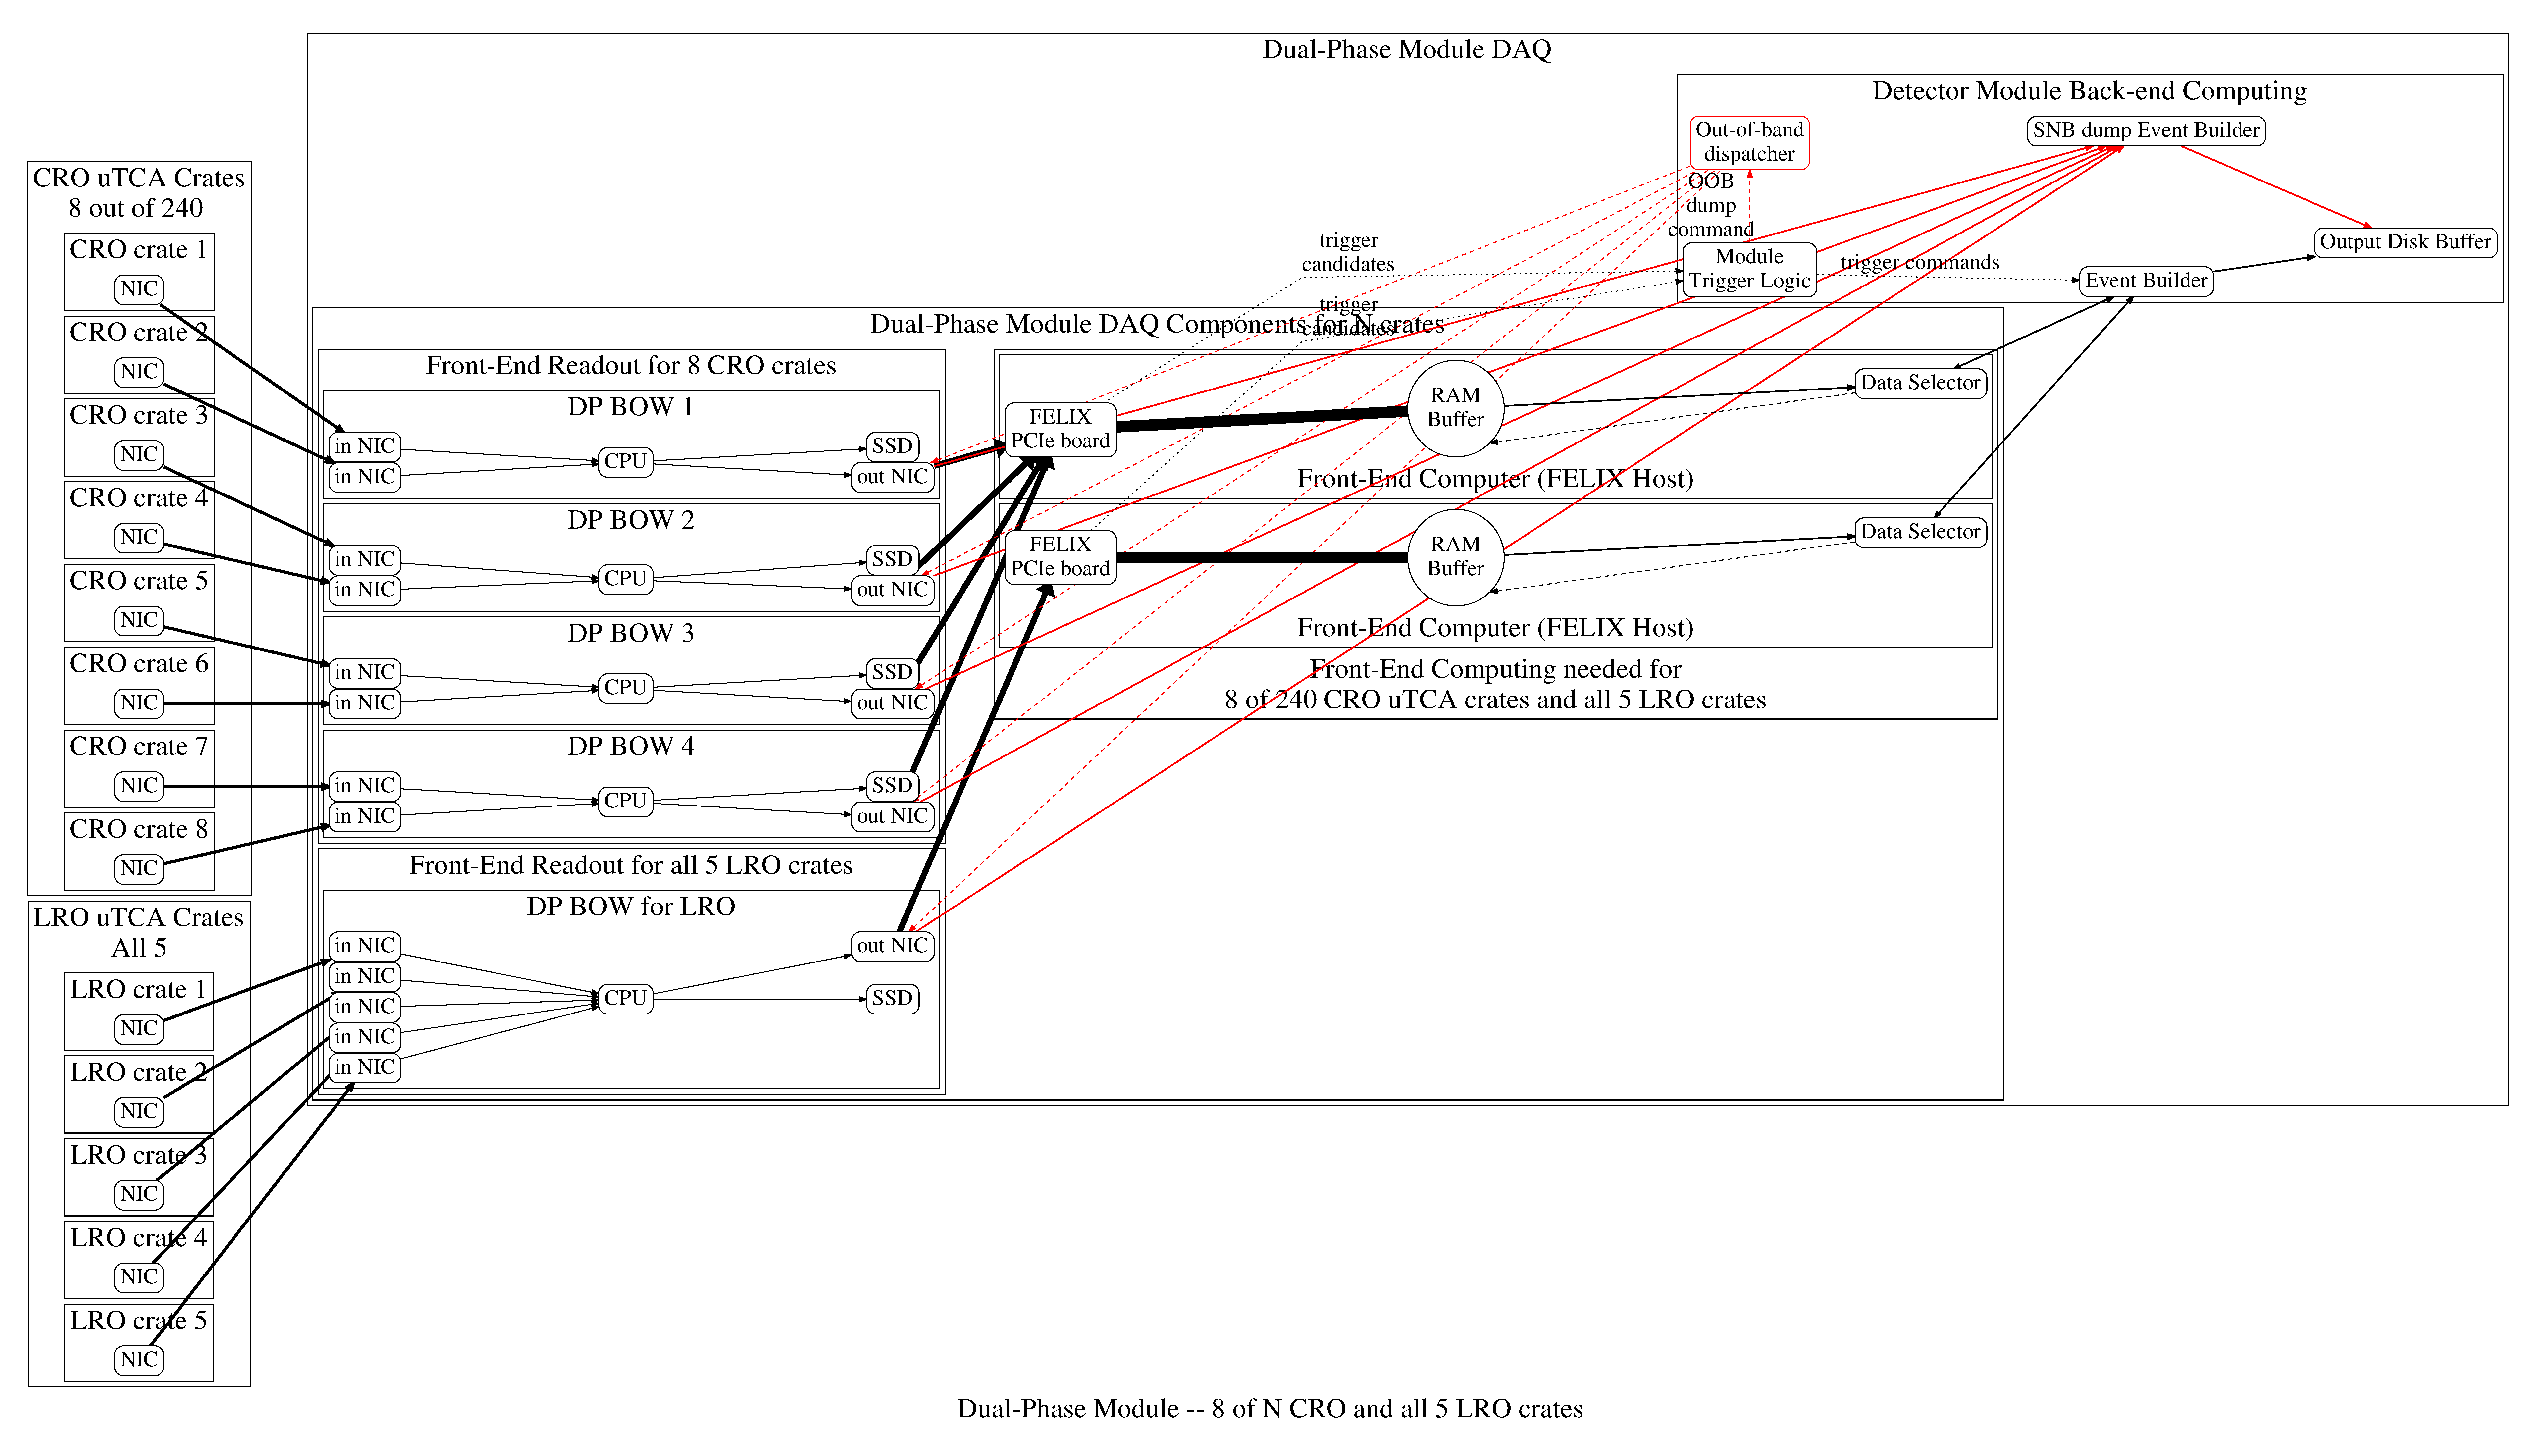
\includegraphics[width=0.8\textwidth]{daq-readout-buffering-baseline.pdf}%
\end{dunefigure}


%%%%%%%%%%%%%%%%%%%%%%%%%%%%%%%%%%%
\subsection{Local Trigger Primitive Generation (Josh Klein \& J.J. Russel \& Brett Viren \& DP Expert?)}
\label{sec:fdsp-daq-ltp}


\Dwords{trigprimitive} are generated inside the \dword{fe} readout
hardware local to each APA from TPC data on a per-channel basis.
They are sent along with the waveform data to the \dword{fe} DAQ
computing where they may be further processed before being sent out to
the \dword{mtl} as \dwords{trigcandidate}.  
Section~\ref{sec:fdsp-daq-sel} describes the selections involved in
this triggering.

Only the 480 collection channels associated with each APA face are
used for forming \dwords{trigprimitive}. 
Reasons for this limitation include the fact that collection
channels:

\begin{itemize}
\item have higher signal to noise ratio compared to induction channels.
\item are fully and independently sensitive to activity on their APA face.
\item have unipolar signals that directly give an approximate measure
  of ionization charge without costly computation required to
  deconvolve the field response functions as required to make use of
  the induction channels..
\item can be easily divided into smaller, independent groups in order
  to better exploit parallel processing.
  % fixme: do we need a statement about efficiency here?
\end{itemize}


Figure~\ref{fig:daq-readout-buffering-baseline} illustrates the connectivity between the
four connectors on each of the five WIBs and the \dword{fe} readout hardware.
The data is received via 80 1 Gbps fiber optical links by four \dwords{rce}
in the \dword{acta} \dword{cob} system. \fixme{Matt: help!  Each RCE consists of a ....}

The pattern of connectivity between WIBs and RCEs results in the data
from the collection channels covering one contiguous half of one APA
face being received by each \dword{rce}.
Each \dword{rce} has two primary functions. 
The first is transmission of all data as described in
Section~\ref{sec:fdsp-daq-hlt}. 
The second is to produce \dwords{trigprimitive} from its portion of the
collection channel data.
The algorithms to produce the \dwords{trigprimitive} still require
development but can be broadly described.   

\begin{enumerate}
\item On a per channel basis calculate a rolling baseline and spread
  level which characterizes recent noise behavior such that the result
  is effectively free of influence from actual ionization signals.
\item Locate contiguous runs of ADC samples that are above a threshold
  defined in terms of the baseline and noise spread.
\item Emit their time bounds and total charge as a \dword{trigprimitive}.
\end{enumerate}

These \dwords{trigprimitive} represent possible activity occurring in
the LAr in a contained by a rectangular volume spanning the height of
the TPC, within half a wire pitch across and which extends in the
drift direction by the time bounds. 
Depending on the threshold set, these \dwords{trigprimitive} may be
numerous due to \Ar39 decays and noise fluctuations.
If their rate can not be sustained, the threshold may be raised or
further processing may be done still at the APA level and which
considers more global information.
This may be performed either in the \dwords{rce} or later in the
\dword{fe} computing hosts. 
In either case, the results are in the form of \dwords{trigcandidate}
which are sent to the \dword{mtl}.

Sources of \dword{rf} emission inside the cryostat are minimized by
design. 
Any residual \dword{rf} is expected to be picked up coherently across
some group of channels. 
Depending on its intensity, additional processing of the collection
waveforms must be employed to mitigate this coherent noise and this
must occur before the data is sent for \dword{trigprimitive}
production. 
If the required mitigation algorithms outgrow the nominally specified
\dword{rce} \dword{fpga} it is possible to double the number of
\dwords{cob} per APA which will require a redistribution of fibers. 
Alternatively, or in addition, the higher number of
\dwords{trigprimitive} produced as a result of excess noise can be
passed along for further processing in the \dword{fe} computing. 
This will require reprocessing the raw waveform data.



%%%%%%%%%%%%%%%%%%%%%%%%%%%%%%%%%%%
\subsection{Dataflow, Trigger and Event Builder (Giles Barr \& Josh Klein \& Giovanna Miotto \& Kurt Biery \& Brett Viren)}
\label{sec:fdsp-daq-hlt}

\metainfo{Describe the dataflow {\it infrastructure}. This should cover transport of data and trigger information, infrastructure for generating local and global trigger commands (but not their algorithms, that's next), as well as what happens to the data once a trigger is generated (ie. event building).
Figure~\ref{fig:daq-readout-buffering-baseline} may be referenced}

The data volume that is continuously flowing through the DUNE
\dword{sp} \dword{detmodule} DAQ from one APA is about \SI{10}{\GB/\s}
and from the entire far detector as much as \SI{10}{\TB/\s}.
However, by design a distributed system that follows the natural
granularity of the detector this high rate data is made manageable.
In particular the \dword{ringbuffer} is defined at the APA level for
the \dword{sp} \dword{detmodule}.
The majority of the data corresponds to the untriggered parts and
never leaves the computers hosting the \dwords{ringbuffer}.
The parts that exit do so in one of three circumstances: (a) as data
selected by nominal \dwords{trigcommand}, (b) as \dwords{trignote} or
(c) as previously triggered \dword{snb} candidate data which is
sent out after being dumped to the SSD storage local to
\dwords{rce} and as available bandwidth permits. 
All three of these transfers live entirely in the software domain of a
commodity computer farm and so a variety of techniques can be
considered for each; in this description, we consider each of them as
a data-pull protocol, similar to that in use at ProtoDUNE.
\fixme{Is it true? 
  There has been the statement that SNB dumps will egress via special
  paths direct to a special EB and not via FELIX. 
  If this isn't the case then figure 7.2 needs fixing.}


artDAQ is a modern, general-purpose framework that has been used in
DUNE prototype tests and elsewhere [refs]. 
It is optimised further than other frameworks to expliot the
paralelism that is possible with modern multi-core machines. 
It is the principle architecture that will be used in DUNE.
\fixme{Context here is too vague. 
  ``...used in DUNE DAQ back-end computing''?}
The authors of artDAQ have accomodated DUNE-specific feature-addition
requests and a number of libraries have been developed based on
existing parts of artDAQ used to handle incoming data from data
sources. 
It is likely that future DUNE extensions will be by one of these two
routes.

(Section on FELIX data ingress, error handling, synchronisation,
ring-buffer expiry). 
As noted above, one of the complex data flow control tasks is managing
the data as it enters the \dwords{ringbuffer} on the per-APA \dword{fe}
computing hosts. 
Data throughput on these nodes is governed by the use of the PCIe and
memory busses, and so the software will be written to mimumize
data-copies on the input side of the \dword{ringbuffer}.
%% removed: this is RCE-land, not primary buffer.
%During normal operation, there must be sufficient 'headroom' to allow
%an additional write of data to SSDs during the supernova burst. 
The current model for dataflow control is that each APA will operate
semi-autonomously, data being written directly from hardware into physical
memory and not moved. 
The software will keep track of the free and in-use memory (one way is
with a ring for each data source) and will maintain an index of the
data. 
One strategy that decentralises the error handling is for the writing
to the \dword{ringbuffer} to not cause error handling events, but
for it to flag areas of the data for which problems exist only if/when
it is to be read again. 
Similarly, to avoid memory alloction error handling, the incoming data
can overwrite the older data and read requests for data that has been
overwritten will report the error. 
It is planned to prototype the data transfers for the TDR.

(Section on (a) event building) Requests for event building
(i.e. reading data for succesful triggers from the \dwords{ringbuffer}
will be done using mostly standard features that are now in artDAQ. 
An \dword{eb} node is allocated for each trigger to be read and it
then requests portions of data from the \dwords{ringbuffer} for the
data from that event (this read must be initiated by the request, a
difference with the current ProtoDUNE).
If the data is missing (either due to errors when it was first
received, or because the request arrived so late that the data were
overwritten), the request still proceeds but with flags set in the event
header and which are displayed on the operators console.

(Section on (b) trigger farming) As described above, a \dword{fec}
will receive \dwords{trigprimitive} from its associated \dwords{rce}
which identify channels and periods of time where potentially useful
signal exists. 
In most circumstances, this will local information will be sufficient
to form a \dword{trigcandidate} which on its own will lead to a
\dword{trigcommand}.
In other cases, such as SNB activity, \dwords{trigcandidate} from many
\dwords{fec} must be combined to form a \dword{trigcommand}.
This trigger information will be gathered into a block of data
spanning some time period. 
Our default scheme for the dataflow is to use a similar method as
employed in \dword{protodune}, however several others are under study. 
For the former, a trigger farm node is assigned to each time block,
requests the associated trigger data block and based on its contents
retrieves the indicated detector data from the appropriate
\dwords{fec}.   
The received detector data is then aggregated along with the
associated trigger information into a \dword{rawevent} (using artDAQ
functions).
Scaling methods are being considered to mitigate bottlenecks as may be
required.  
These are based adding an intermediate layer which groups a number of
\dwords{fec} to avoid the possibility of too many small blocks of
data.
\fixme{This next sentence doesn't make sense: ``Another solution is
  to use data-push, since, it is likely that a single node with a lot
  of cores can deal with all the trigger processing.''}

\fixme{We need something about running in a partitioned mode. 
  Eg, 148 APAs working nominally and 2 in their own partition for the
  purpose of calibration or debugging or something.}

(Section on (c) SNB trickling) The average rate of dump
\dwords{trigcommand} such as may be issued by a SNB candidate will be
relatively low. 
The nominal period of the dump is \SI{10}{\s} which will thus produce
about \SI{15}{\TB} across the entire \dword{sp} \dword{detmodule}. 
Spread over the 600 \dword{ssd} units this leads to about \SI{25}{\GB}
per \dword{rce} per dump. 
Today, typical \dwords{ssd} offer storage on the order of \SI{1}{\TB}. 
For any reasonable SNB false-positive trigger rate, there will be
sufficient \dword{ssd} capacity to store dumps for years and to not
directly drive any throughput requirements on the DAQ.
It is thus expected that this dump data will be sent out as a
background process. 
The SNB event building will likely differ somewhat from nominal in
that the entire dump will not be held in a single \dword{rawevent}
object as this would produce a single \SI{15}{\TB} file.


%%%%%%%%%%%%%%%%%%%%%%%%%%%%%%%%%%%
\subsection{Data Selection Algorithms (Josh Klein \& Brett Viren)}
\label{sec:fdsp-daq-sel}

%This section describes the strategy for using the trigger/dataflow infrastructure, with example algorithms.

\fixme{Need to add Josh's table of data volumes.}

Data Selection will follow a hierarchical design. 
It begins with forming local, APA-level \dwords{trigcandidate} which
are used to form \dword{detmodule} \dwords{trigcommand} in the
\dword{mtl} which lead to readout of a small subset of the total data. 
In addition, \dwords{trigcandidate} will be provided to the
\dword{mtl} from external sources such as the \dword{gtl} in order to
indicate external events such as beam spills, or SNB candidates
detected by the other \dwords{detmodule} or by SNEWS.
A \dword{hlt} may also be active within the \dword{mtl}. 
The hierarchical approach is both natural from a design standpoint, as
well as allowing for vertical slice testing and partitioning during
commissioning of the system.

As discussed above, \dwords{trigprimitive} will be generated in the
\dwords{rce} from the data stream for each collection channel. 
The \dwords{trigprimitive} will contain summary information for each
collection wire, such as the time of any threshold-crossing pulse, its
integral charge, and time over threshold. 
A collection wire with an associated \dword{trigprimitive} is said to
be ``hit'' for the time spanned by the primitive. 
These trigger primitives are then passed, along with the full data
stream, to the \dword{fec}, each of which handles channels from a pair
of \dwords{apa}. 
An APA-level \dword{trigcandidate} is passed upward to the
\dword{mtl}, which arbitrates between various trigger types,
determines trigger priority and ultimately the time range and detector
coverage for a \dword{trigcommand} which it emits back to the
\dwords{fec}.
The \dword{mtl} assures that no overlapping \dwords{trigcommand} are
issued.
It also may emply a \dword{hlt} to allow for a reduction or an
aggregation of triggers to reduce or optimize the subsequent readout
of high rate activity such as due to various backgrounds, including
instrumental effects, as needed.

A valid \dword{detmodule}-level, single-interaction trigger sends
\dwords{trigcommand} back to the \dwords{fec} telling it which slice
of time should be saved under the particular trigger header. 
At the start of DUNE data taking, it is anticipated that for any given
single-interaction trigger (a cosmic ray track, for example) waveforms
for all wires will be recorded for a full \readout \dword{readout
  window}. 
Such an approach is clearly very conservative, but it ensures that
associated low-energy physics (such as captures of neutrons from
produced by neutrino interactions or cosmic rays) will be recorded
without any need to fine-tune APA-level triggering, and will not
depend on the noise environment across the APAs. 
In addition, the \readout readout window ensures that regardless of when
a given even causes a trigger, the entire track is recorded. 
It is estimated that this generous \dword{readout window} will not
produce an unmanageable data volume. 
We anticipate, however, that as we gain experience running DUNE the
overall data volume will reduced by writing out data from only a
subset of APAs for any given track, and possibly reducing the size of
the readout window.

Other trigger streams---calibrations, random triggers, and prescales
of various trigger thresholds, will also be generated at the
\dword{detmodule} level, and filtering and compression can be applied
based upon the trigger stream. 
For example, a large fraction of random triggers may have \dword{zs}
applied to their waveforms, reducing the data volume substantially, as
the dominant data source for these will be $^{39}$Ar events.
Additional signal-processing can also be done on particular trigger
streams if needed and if the processing is available, such as fast
analyses of calibration data.

At the \dword{detmodule} level, a decision can also be made on whether
a series of interactions are consistent with a \dword{snb}. 
If the number of \dword{apa} level, low-energy \dwords{trigcandidate}
exceeds a threshold for the number of such events in a given time, a
trigger command is sent from the \dword{mtl} back to the \dwords{rce},
which store up to \SI{10}{\s} of unsuppressed, full waveform data. 
That full waveform is then written out as a separate trigger stream
for fast analysis by the supernova working group, perhaps as an
automated process. 
In addition, the \dword{mtl} passes information about APA level
\dwords{trigcandidate} up to a detector-wide \dword{gtl}, which among
other functions can decide whether, integrated across all modules,
enough APAs have detected interactions to qualify for a \dword{snb}
even if within a particular module the threshold is not exceeded. 
\Dwords{trigcandidate} from the \dword{gtl} are passed to the
\dword{mtl} for dispatch to the \dwords{fec} (or \dwords{rce} in the
case of SNB dump commands). 
That is, to the \dword{mtl}, an \dword{externtrigger} looks like just
one more ``external'' trigger input.

APA level \dwords{trigcandidate} will be generated within each server
of the \dwords{fec}. 
The trigger decision will be based on the number of adjacent
collection wires hit in a given APA within a time window (roughly
\SI{100}{\us}), the total charge on these adjacent wires (or possibly
on any hit wire in the collection plane), and possibly the union of
time-over-threshold for the \dwords{trigprimitive} in the collection
plane.
Our studies show that even for low-energy events (roughly
\SIrange{10}{20}{\MeV}) the reduction in radiological backgrounds is
extremely high with such criteria.
The highest-rate background, $^{39}$Ar, which has a decay rate of
10~MBq within a \SI{10}{\kton} volume of argon, has an endpoint of 500
keV and requires significant pileup in both space and time to get near
a \SI{10}{\MeV} threshold.
Other important background sources are $^{42}$Ar, which has a 3.5 MeV
endpoint and a decay rate of 1 kBq, and $^{222}$Rn which has a decay
rate of XXXX and decays via a highly-quenched $\alpha$ of 5.5 MeV.
\fixme{Need Rn-222 decay rate.}
The radon decays to $^{218}$Po which a few minutes later leads to a
quenched $\alpha$ of 6 MeV, and ultimately a $^{214}$Bi daughter (many
minutes later) which has a $\beta$ decay with endpoint near 3.5 MeV. 
The $\alpha$ ranges are short and will hit at most a few collection
wires, but the charge deposit can be large, and therefore the charge
threshold will have to be well above the $\alpha$ deposits plus any
pileup from $^{39}$Ar and noise.

At the APA level, two kinds of local \dwords{trigcandidate} can be
generated.
One is a ``high-energy'' trigger, that indicates that within a given
APA a candidate event with energy more than \SI{10}{\MeV} has been
found.
The thresholds in hit wires, total charge, and time-over-threshold,
will be optimized for at least 50\% efficiency at this threshold, with
efficiency increasing to 100\% via a turn-on curve that ensures at
least 90\% efficiency at \SI{20}{\MeV}. 
A second APA level trigger candiate will be generated for low-energy
events, between \SI{5}{\MeV} and \SI{10}{\MeV}. 
These low-energy APA trigger candidates will not by themselves
generate valid \dword{detmodule} level triggers, but rather be used at
the \dword{detmodule} level to determine whether a burst of events
across many APAs is consistent with a supernova.

The \dword{detmodule} level takes as input both APA level
\dwords{trigcandidate} (both low-energy and high-energy), as well as
\dword{externtrigger} sources, such as the \dword{gtl} which includes
global, detector-wide triggers, external trigger sources such as
SNEWS, and information about the time of a Fermilab beam spill. 
The \dword{mtl} will also generate internal triggers, such as random
triggers and calibration triggers (for example, telling a laser system
to fire at a prescribed time). 
In addition, at the \dword{mtl} prescales of all trigger types that
normally would not generate a \dword{trigcommand} will be made. 
For example, a single low-energy \dword{trigcandidate} does not cause
a \dword{trigcommand} on its own, but at some large prescale fraction
it could.


The \dword{mtl} is responsible also for checking candidate triggers
against the current \dword{rc} trigger mask: in some runs, for
example, we may decide that only random triggers are accepted, or that
certain APA trigger candidates should not be accepted because those
APAs are noisy or misbehaving in some way. 
In addition, the \dword{mtl} will count low-energy trigger candidates
from the APAs and, based upon the number and distribution of those
triggers in a long time interval (e.g., \SI{10}{\s}), decide to
generate a \dword{snb} trigger command.
 The trigger logic will be
optimized to record the data due to at least 90\% of all Milky Way
supernovae, and our studies of simple low-energy trigger criteria show
that we can likely do much better than that.  

	
The \dword{hlt} can also be applied at this level, particularly if
there are unexpectedly higher rates from instrumental or low-energy
backgrounds, that require some level of reconstruction or pattern
recognition. 
An \dword{hlt} might also allow for efficiently triggering on
lower-energy single interactions, or allow for better sensitivity for
supernovae beyond the Milky Way, by employing a weighting scheme to
individual APA level \dwords{trigcandidate}---higher-energy
\dwords{trigcandidate} receiving higher weights. 
Thus, for example, two APA level \dwords{trigcandidate} consistent
with \SI{10}{\MeV} interactions in \SI{10}{\s} might be enough to
create a \dword{snb} candidate trigger, while 100 \SI{5}{\MeV} APA
level trigger candiates in \SI{10}{\s} might not.
Lastly, the \dword{hlt} can allow for dynamic thresholding; for
example, if a trigger appears to be due to a cosmic-ray muon, the
threshold for single interactions can be lowered (and possibly
prescaled) for a short time after that to identify spallation
products. 
In addition, the \dword{hlt} could allow for a dynamic threshold after
a \dword{snb}, to extend sensitivity beyond the \SI{10}{\s}
\dword{snb} \dword{readout window}, while not increasing the data
volume associated with \dword{snb} candidates linearly. 

All low-energy \dwords{trigcandidate} are also passed upwards to the
\dword{gtl}, which can integrate the APA level trigger across all
\SI{10}{\kton} \dwords{detmodule} and determine if enough APAs have
\dwords{trigcandidate} that a \dword{snb} may be occuring. 
This approach increases the sensitivity to trigger on bursts by a
factor of four (for \SI{40}{\kton}), thus extending the burst
sensitivity to a distance twice as far as for a single \SI{10}{\kton}
\dword{detmodule}. 

	
The \dword{mtl} is also responsible for creating a trigger header that
includes a global timestamp for the trigger from its input
\dwords{trigcandidate}, and information on what type of trigger was
created. 
A log of all APA level \dwords{trigcandidate} will also be kept,
whether or not they contribute to the formation of a
\dword{trigcommand}. 
As described above, the \dword{readout window} for nominal
\dwords{trigcommand} (those other than for \dword{snb} candidates) is
\readout.
Thus, a nominal DUNE ``event'' is \readout of data from all wires
in the \dword{sp} \dword{detmodule} in response to a \dword{mtl}
\dword{trigcommand}. 
The \dword{mtl} is also responsible for sending the trigger commands
that tell the RCEs to dump their \SI{10}{\s} ``supernova'' buffer. 
If a supernova burst trigger is created at the \dword{gtl} level, an
\dword{externtrigger} is passed back down to the \dword{mtl}, which
then dispatches a dump \dword{trigcommand} to the RCEs for readout of
the long (\SI{10}{\s}) unsuppressed buffer, the same way it would if a
supernova burst is detected at the \dword{mtl}.

\fixme{There are still a lot of repetition of concepts and statements in the above section.}

	


%\metainfo{Describe Module Trigger Logic and Global Trigger Logic.
%  Describe creation of Trigger Command Messages (TCM) from TPMs.
%  Included external sources of TPMs such as SNEWS, Fermilab Beam,
%  testing triggers, periodic triggers, calibration triggers.}
%
%\metainfo{Here should go the assumptions that went into the thinking
%  for Josh's event category data volumes.  It can include discussion
%  of tighter selection criteria for ``cosmics'' such as Phil's
%  distribution of number of APAs hit by cosmics and arguments for
%  something less than 2+ drift time readouts.}

%
% %%%%%%%%%%%%%%%%%%%%%%%%%%%%%%%%%%%
% \subsection{High-Level Trigger}
% \label{sec:fdsp-daq-eb}
%
% Data selection after event building.
%

\subsection{Timing \& Synchronization (David Cussans \& Kostas Manolopoulos)}
\label{sec:fdsp-daq-timing}

%Describe the generation of timing/synchronisation signals and and distribution to the detectors.

All components of the DUNE \dword{sp} \dword{detmodule} are
synchronized to a common clock.  In order make full use of the
information from the photon detection system the common clock must be
aligned within a single \dword{detunit} with an accuracy of O(1ns).
In order to form a common trigger for \dword{snb} between
\dwords{detmodule} the timing between them must be aligned with an
accuracy of O(1ms).  However, a tighter constraint is the need to
calibrate the common clock to universal time (derived from GPS) in
order to adjust the data selection algorithm inside an accelerator
spill, which requires an absolute accuracy of O(1us).

Single and Dual phase detector modules use a different timing system,
driven by the different technical requirements and development history
of the two systems. A single phase detector module has many more
timing end-points than a dual phase module and many of the end-points
are simpler than the end-points in the dual phase, for example a WIB
vs. uTCA crate. Both systems have been sucessfully prototyped.

The DUNE \dword{sp} \dword{detmodule} uses a development of the protoDUNE
timing system. Synchronization messages are transmitted over a serial
data stream with the clock embedded in the data. The format is
described in DUNE DocDB-1651. Figure~\ref{fig:daq-readout-timing}
shows the overall arrangement of components within the Single Phase
Timing System(SPTS). A stable master clock, disciplined with a \SI{10}{\MHz}
reference is used in the SPTS. A \dword{pps} is
also received by the system and is time-stamped onto a counter clocked
by the SPTS master clock, however the periodic synchronization
messages distributed to the \dword{sp} \dword{detmodule} are an exact number
of clock cycles apart even if there is jitter in the \dword{pps}.
\fixme{Need reference added for DocDB-1651.}

The GPS signal is encoded onto optical fibre and transmitted to the
CUC, where it is converted back to an RF signal on coaxial cable and
used as the input to a GPS displined oscillator. The oscillator module
also houses a IEEE 1588 (PTP) Grand Master and an NTP server. The PTP
Grand Master provides a timing signal for the \dword{dp} White Rabbit
timing network. The NTP server provides an absolute time for the
\dword{pps}. The SPTS relates its time counter onto GPS time by
timestamping the \dword{pps} onto the SPTS time counter and reading
the time in software from the NTP server.

The latency from the GPS antenna on the surface to the GPS receiver in
the CUC will be measured by optical time domain reflectometry at
installation. Given the modest absolute time accuracy required
(sufficient to select data within an accelerator spill) dynamic
monitoring of this delay is not required.

The White Rabbit synchronization signals from the \dword{dp} \dword{detmodule} are
time-stamped onto the SPTS clock domain and the SPTS synchronization
signals are time stamped onto the \dword{dp} clock domain. This allows
the timing in the \dword{sp} and \dword{dp} detectors to be
aligned. A similar scheme is used to relate the \dword{sp} protoDUNE
\dword{sp} timing domain to be related to the beam instrumentation
White Rabbit time domain.

In order to provide redundancy, and also the ability to easily detect
issues with the timing path, two independent GPS systems are used. One
with an antenna at the head of the Yates shaft, the other with an
antenna at the head of the Ross shaft. The two independent timing
paths are brought together in the same rack in the CUC. Using 1:2
fibre splitters one SPTS unit can be left as a hot-spare while the
other is active. This also allows testing of new firmware and software
during comissioning without the risk of loosing the SPTS if a bug is
introduced.


\begin{dunefigure}[Arrangement of Components in DUNE Timing System]{fig:daq-readout-timing}
  {Illustration of the components in the DUNE Timing System.}
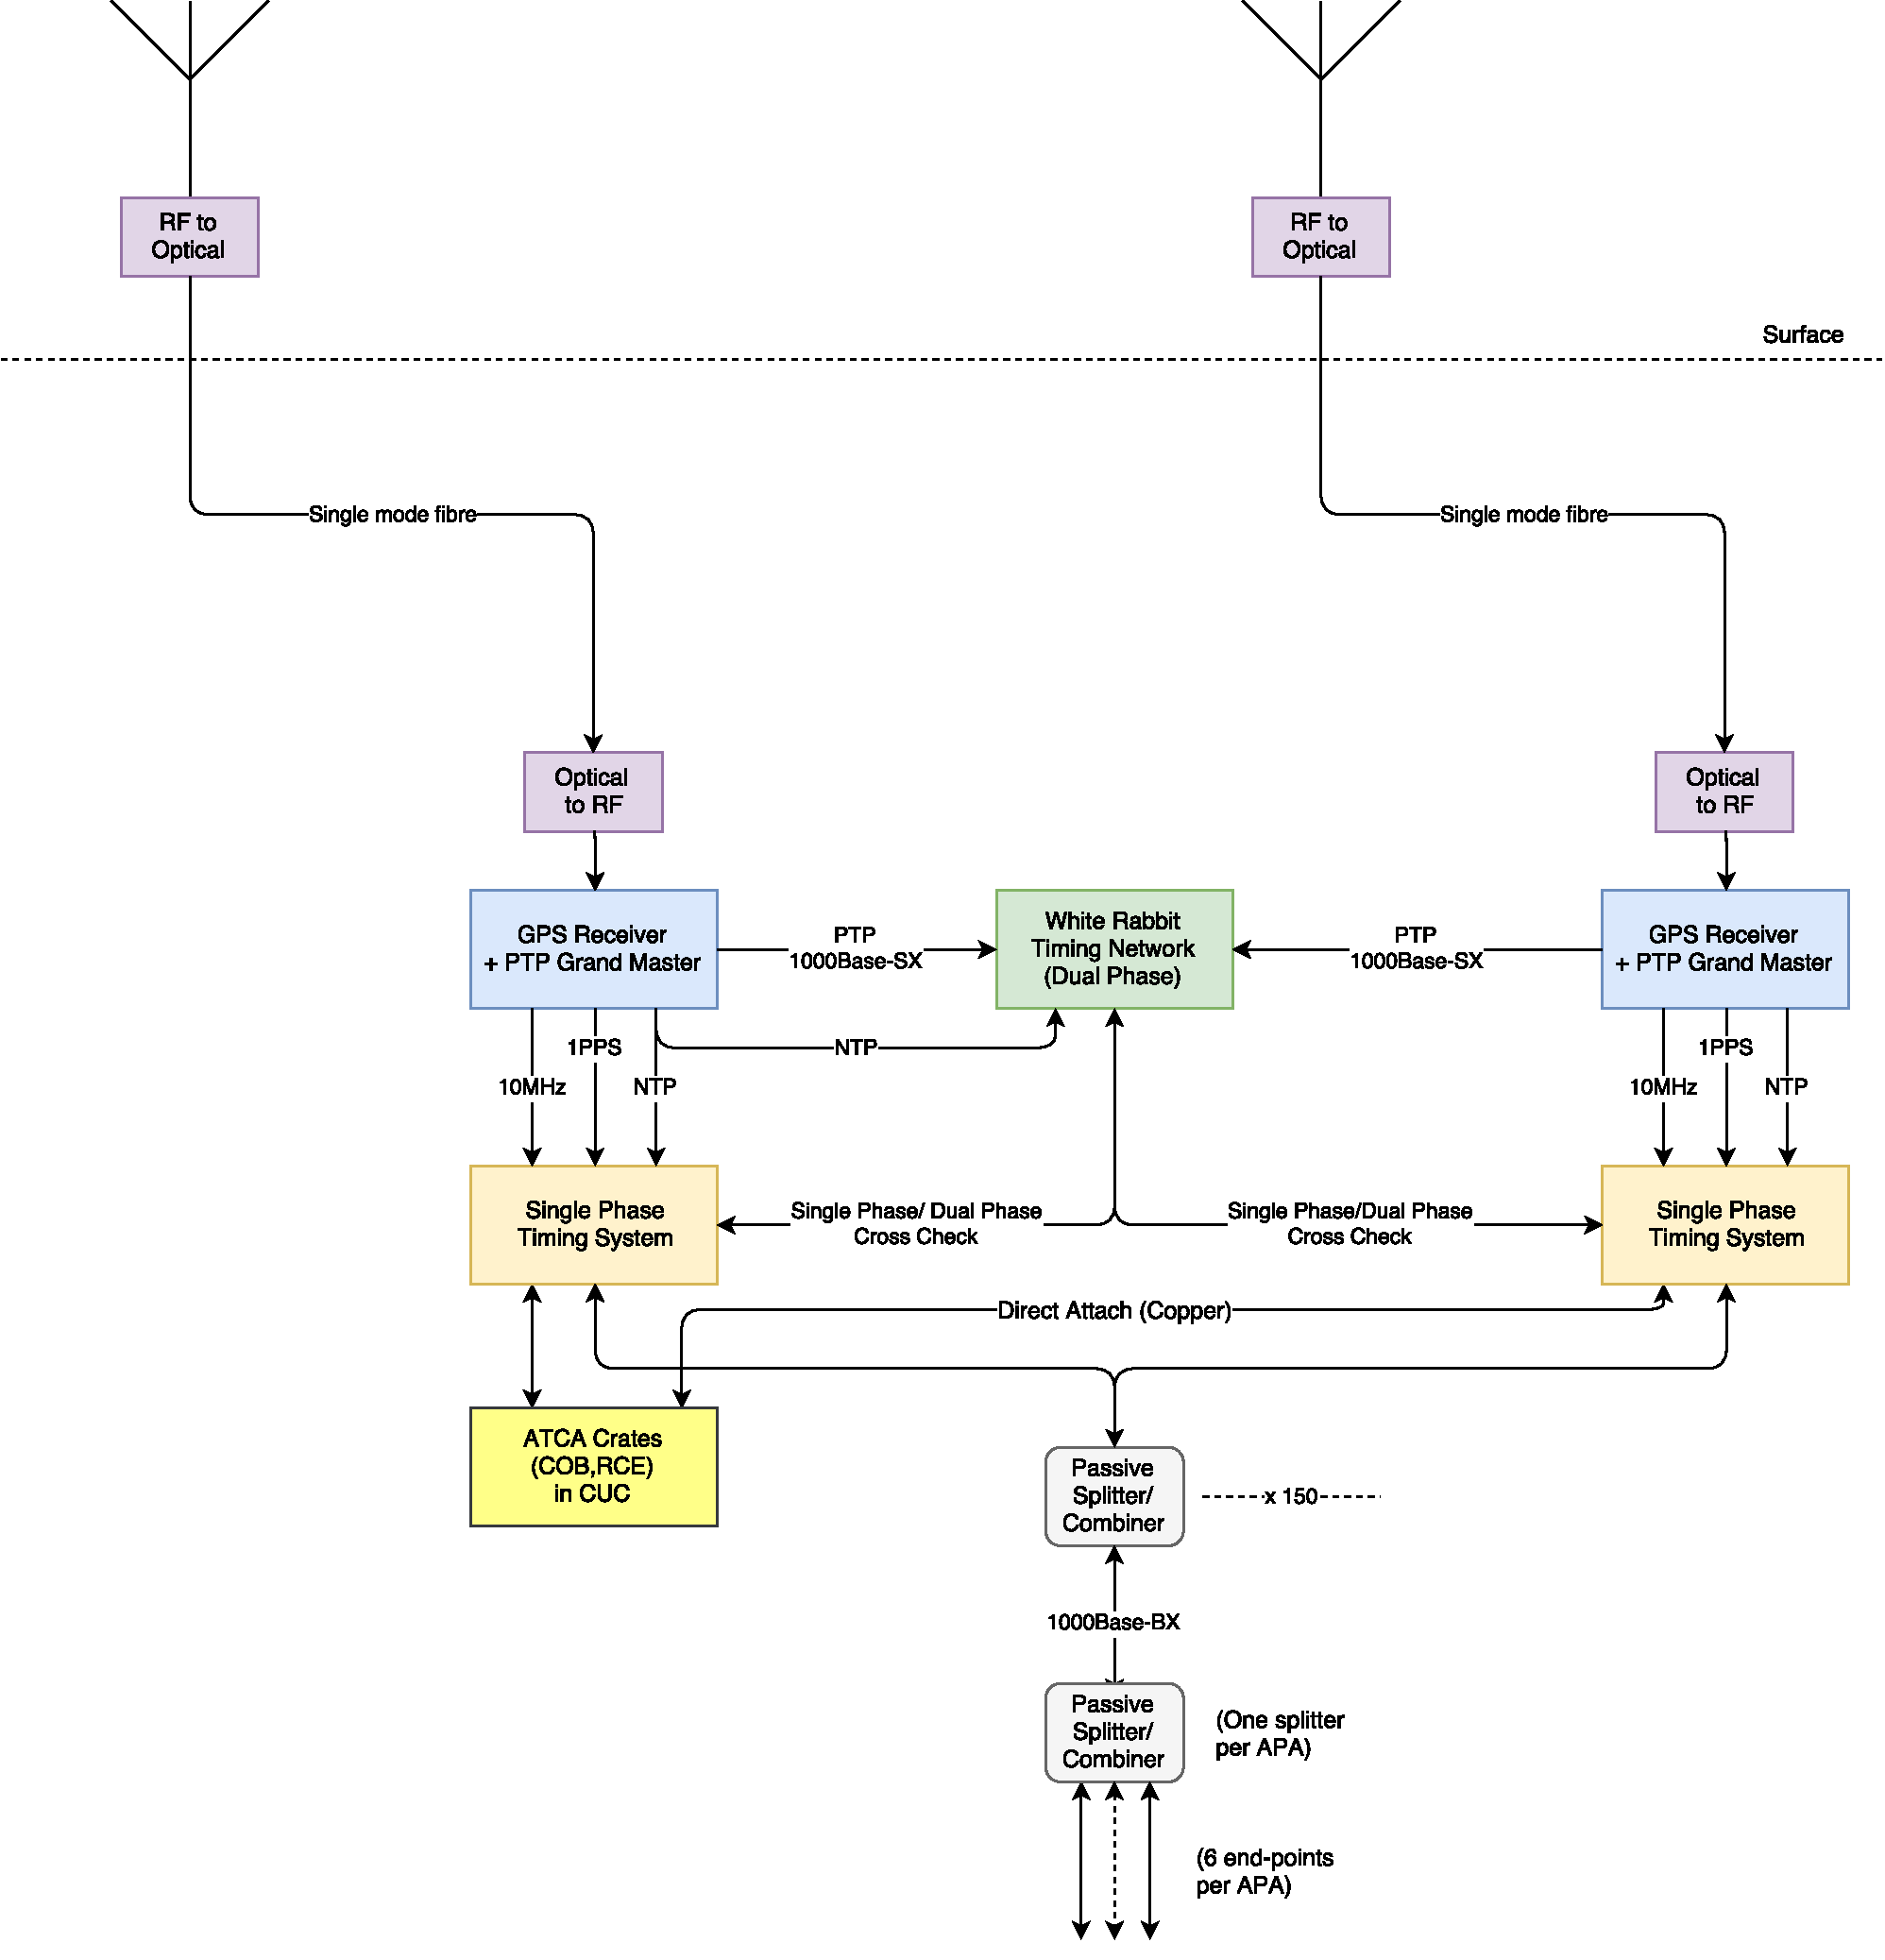
\includegraphics[width=0.8\textwidth]{DUNE_Timing_overall.pdf}
\end{dunefigure}

All the custom electronic components for the SPTS are contained in two
Micro-TCA shelves. At any one time one is active and the other is a
hot-spare. The \SI{10}{\MHz} reference clock and the \dword{pps} are received
by a single width AMC at the centre of the Micro-TCA shelf. This
master timing AMC produces the SPTS signals and encodes them onto a
serial data stream. This serial datastream is distributed over a
standard star-point backplane to the fanout AMCs which each drive the
signal onto up to 13 SFP cages. The SFP cages are either occupied by
1000Base-BX SFPs, each of which connects to a fibre running to an APA,
or to a Direct Attach cable which connects to systems elsewhere in the
CUC, i.e. the \dword{rce} crates and the data selection system. This
arrangement is shown in figure \ref{fig:daq-readout-sp-timing}


\begin{dunefigure}[Arrangement of components in \dlong{sp} timing system]{fig:daq-readout-sp-timing}
  {Illustration of the components in the Single Phase Timing System.}
  %\fixme{Add a diagram of the SPTS electronics}
  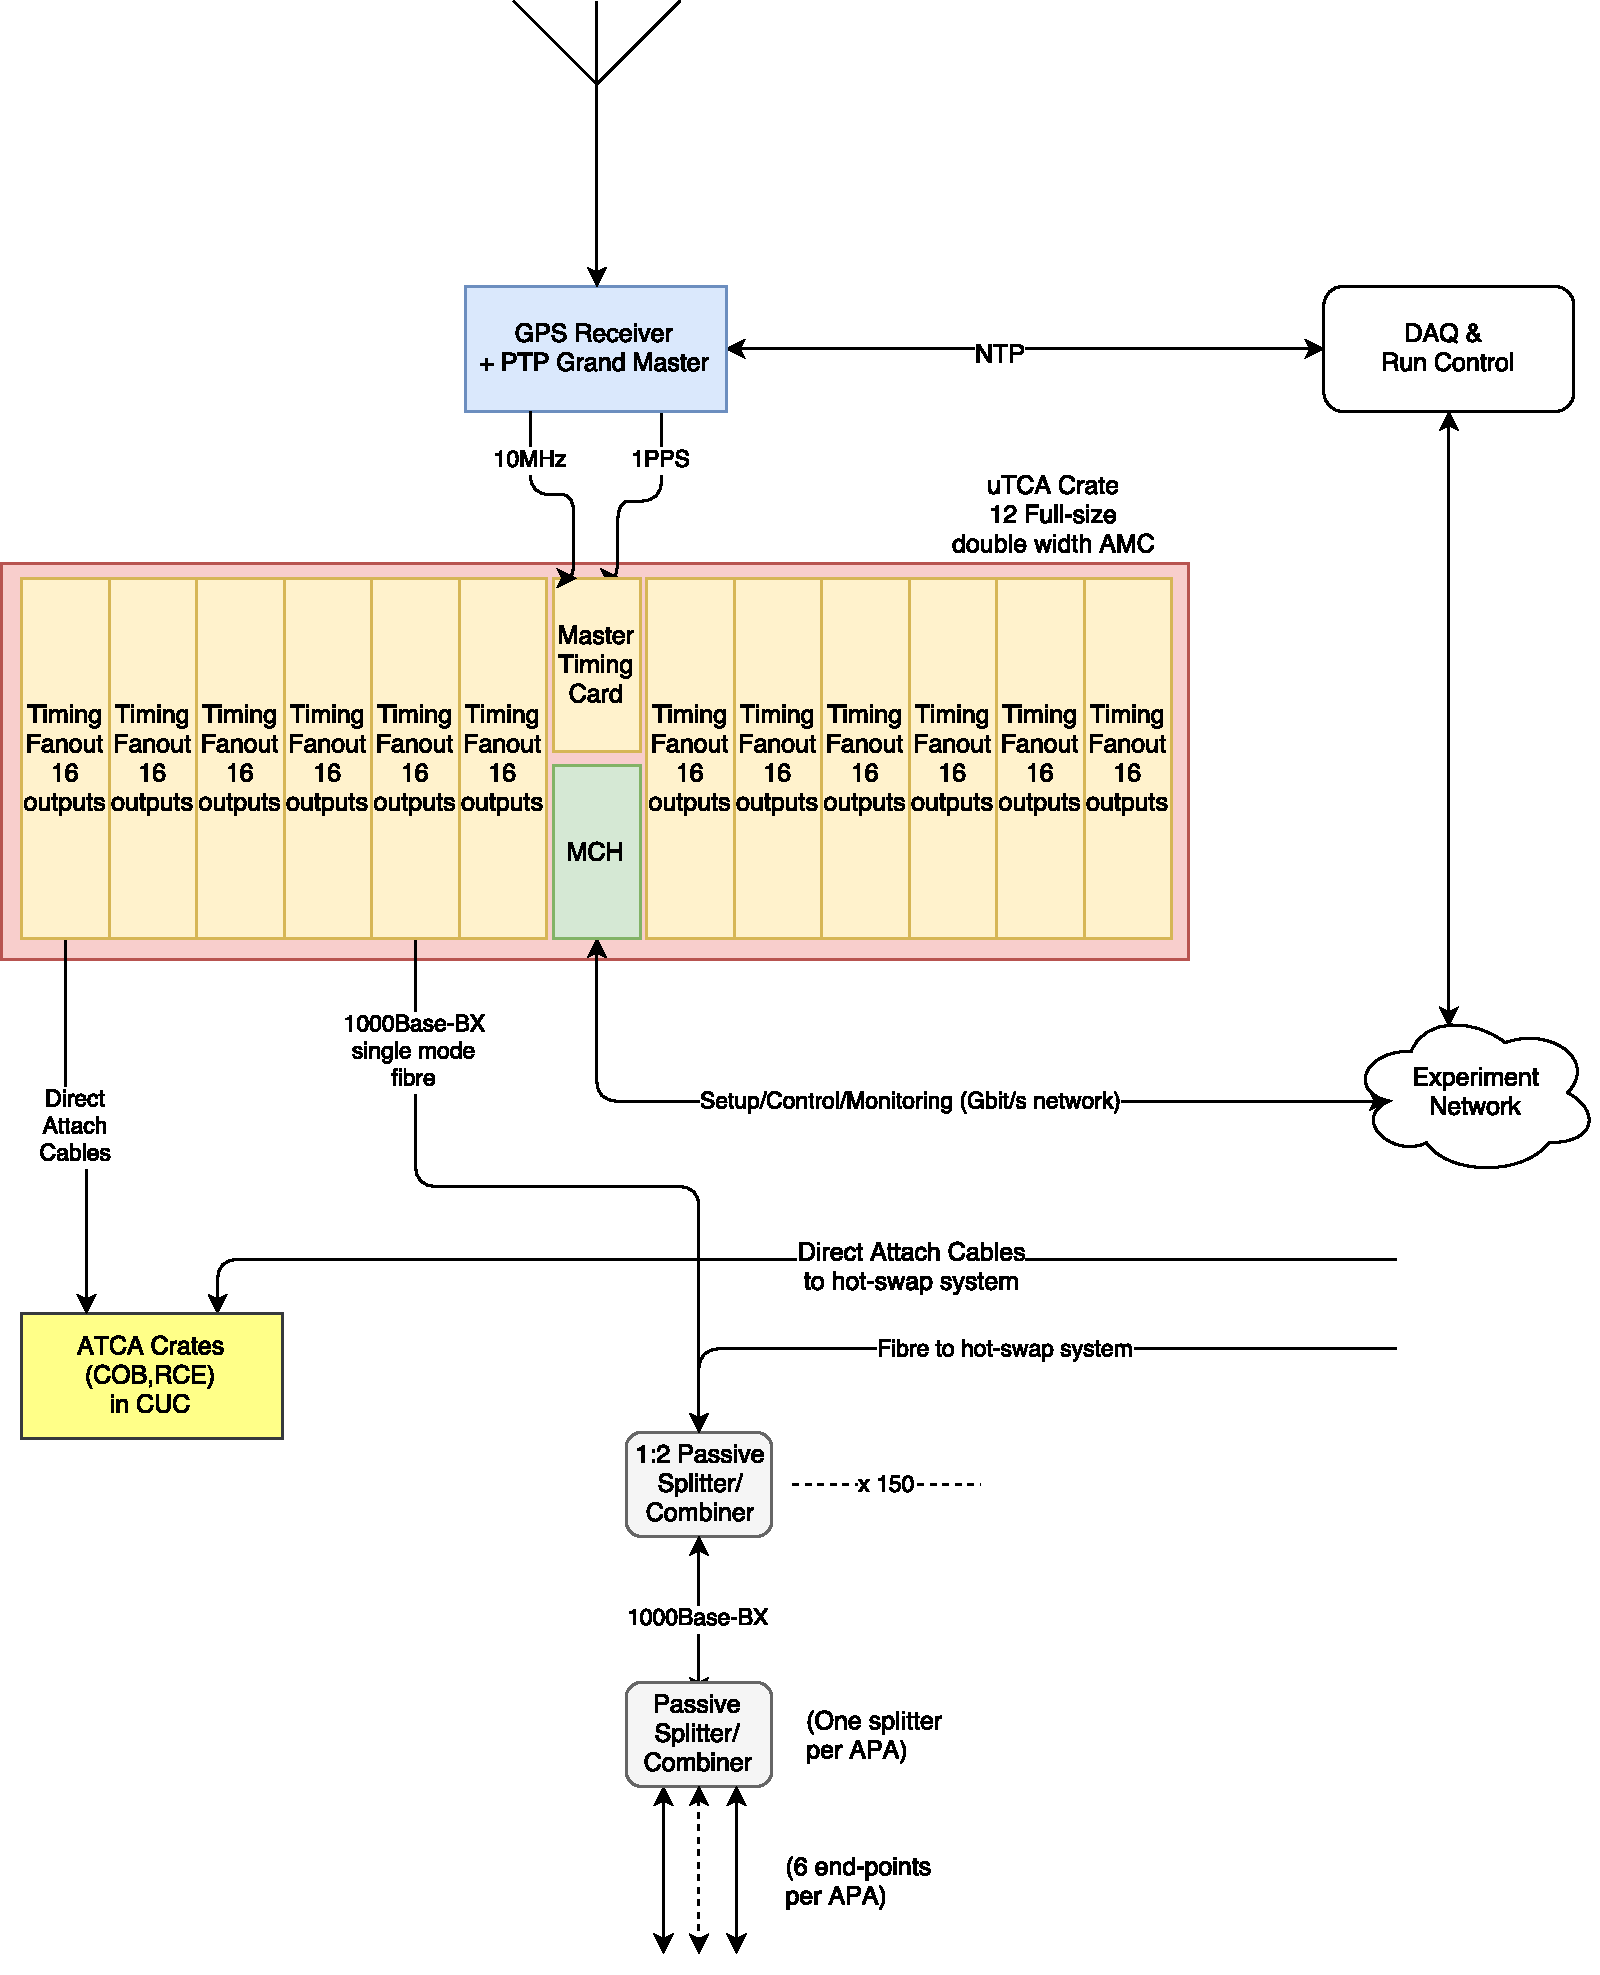
\includegraphics[width=0.8\textwidth]{DUNE_SP_Timing.pdf}
\end{dunefigure}

\subsubsection{Beam timing}
\label{sec:fdsp-daq-design-beamtiming}

The neutrino beam is produced at the Fermilab accelerator complex in
spills of \SI{10}{\us} duration.  A \dword{sls} at the far
detector site will locate the time periods in the data when beam could
be present, based on network packets received from Fermilab containing
predictions of the GPS-time of the spills.  Experience from
MINOS and NOvA shows that this can provide beam triggering with high
reliability, although the system outlined here contains an extra layer
of redundancy in this process.  Several stages of narrowing down the
window in which the beam arrives will be done, aiming for an accuracy
of better than 10\% of a readout time (\readout) at the time the data
are selected from the DAQ buffers.  Ultimately, an offline database
will match the actual time of the spill with the data, thus removing
any reliance on real-time network transfer for this crucial stage of
the oscillation measurements, the network transfer of spill-timing
information is simply to ensure a correctly located and sufficiently
wide window of data is considered as beam data. This system is not
required, and is not designed to provide signals accurate enough to
measure neutrino time-of-flight.

The precision to which the spill time can be predicted at Fermilab
improves as the acceleration process of the protons producing the
spill in question advances.  The spills currently occur at intervals
of \SI{1.3}{\s}; the system will be designed to work with any interval, and
to be adaptable in case the sequence described here changes.  For
redundancy, three packets will be sent to the far detector for each
spill.  The first is approximately \SI{1.6}{\s} before the spill-time, which
is at the point where a \SI{15}{\Hz} booster cycle is selected; from this
point on, there will be a fixed number of booster cycles until the
neutrinos and the time is subject to a few ms of jitter.  The second
is about \SI{0.7}{\s} before the spill, at the point where the main injector
acceleration is no longer coupled to the booster timing; this is
governed by a crystal oscillator and so has a few \si{\us} of jitter.
The third will be at the so called `\texttt{\$74}' signal which is just before the beam line kicker magnet fires
to direct the protons at the LBNF target; this doesn't improve the
timing at the far detector much, but serves as a cross check for
missing packets.  This system is enhanced compared to that of
MINOS/NOvA, which only use the third of the above timing signals.  The
reason for the larger uncertainty in the time interval from \SI{1.6}{\s} to
\SI{0.7}{\s} is that the booster cycle time is synchronised to the
electricity supply company's \SI{60}{\Hz} which has a variation of about
1\%.

Arrival-time monitoring information from a year of MINOS data-taking
was analysed, and it was found that 97\% of packets arrived within
\SI{100}{\ms} of being sent and 99.88\% within \SI{300}{\ms}.

The \dword{sls} will therefore have estimators of the GPS-times of
future spills, and recent spills with associated data contained in the
\dwords{ringbuffer}. These estimators will improve in precision as
more packets arrive.  The DAQ will use data in a wider window than
usual, if, at the time the trigger decision has to be made, the
precision is less accurate due to missing or late packets.  From the
MINOS monitoting analysis, this will be very rare.

%%%%%%%%%%%%%%%%%%%%%%%%%%%%%%%%%%%
\subsection{Computing \& Network Infrastructure (Kurt Biery \& Babak Abi)}
\label{sec:fdsp-daq-infra}

The computing and network infrastructure that will be used in each
of the four \dwords{detmodule} will be similar, if not identical.
It will support the buffering, data selection, event
building, and data flow functionality described
above, and it will include computing elements which consist of servers that:

\begin{itemize}
\item buffer the data until a \dword{trigdecision}
  is received
\item host the software processes that
  build the data fragments from the relevant
  parts of the detector into complete events
\item host the processes that make the
  \dword{trigdecision}
\item host the data logging processes and
  the disk buffer where the data is written
\item host the real-time \dlong{dqm} processing
\item host the control and monitoring processes
\end{itemize}

The network infrastructure that will connect these computers
will have the following components:

\begin{itemize}
\item subnet(s) for transferring triggered data from the buffer
  nodes to the event builder nodes.  These will need to
  connect underground and above-ground computers.
\item a control and monitoring subnet that will connect all
  computers in the \dword{daq} system and all front-end
  electronics that support Ethernet communication.  This
  sub-network will need to connect underground and
  above-ground computers.
\item a subnet for transferring complete events from the
  event builder servers to the storage servers.  This subnet
  will be completely above-ground.
\end{itemize}

%%%%%%%%%%%%%%%%%%%%%%%%%%%%%%%%%%%
\subsection{Run Control \& Monitoring (Giovanna Miotto \& Jingbo Wang}
\label{sec:fdsp-daq-tcm}

Describe how the system is controlled and monitored.

